\chapter{Background}
\label{chap:background}
\section{GPU Architecture}

\subsection{CUDA}

NVIDIA's Compute Unified Device Architecture (CUDA) is the dominant proprietary framework used to access and control NVIDIA GPUs.
CUDA provides the toolchain required to create applications that run on the GPU.
As noted earlier, GPUs are coprocessors to CPUs; CPUs must give the instructions to launch a GPU kernel, the body of code that each thread on the GPU runs.
The CUDA engineer writes these kernels to be launched on the GPU.

There are various parameters that one can control when writing and launching a GPU kernel.
The thread model and memory model are the most common of these parameters.
The thread model defines how many and in what configuration a kernel launches its threads.
There are four layers in the CUDA thread model: the grid, the block, the thread, and the warp.
The grid is composed of all the CUDA threads, grouped into blocks.
Various limits are imposed on the dimensions and sizes of these grids and blocks.
These limits depend on the compute capability of the GPU, which closely coincides with the microarchitecture of the GPU.
When launching a kernel, the engineer specifies exactly how many blocks should be launched and how many threads make up each block.
Uncontrolled by the engineer, the warp is a group of threads that execute in lockstep.

The memory model defines the different memory types available to the layers of the thread model.
The first and largest is the global memory.
It is the slowest of all the memory types but is accessible from all of the threads.
Global memory is usually the advertised GPU memory size.
Next is shared memory, which any thread in a block can access.
Shared memory is much faster than global memory, but is limited in size per block.
Lastly, registers are the fastest but are limited to an individual thread.
These limits are also dependant on the compute capability of the GPU and the binary.
The CUDA engineer usually tries to limit their accesses to global memory and make use of the faster shared and register memory.

\subsection{Libraries and Parallel Primitives}
\label{sec:primitives}

A variety of libraries make development on CUDA more streamlined.
Some provide a fast solution to a particular problem.
Others provide layers of abstraction to hide the complexity of CUDA programming.
This includes the transfer of memory and the thread model.
In our implementation, we try and use libraries whenever possible.
First, these libraries have been developed over a long time by people who are more familiar with the architecture and the quirks that come with it.
Second, abstraction allows a problem to be continually optimized, while presenting a common API to use.
This allows us to somewhat future-proof our implementation, since the libraries should be updated in the future against newer CUDA versions and hardware.
Also, some problems may seem simple at first, but too complex to reimplement every time.
Lastly, the purpose of many libraries are to provide solutions to parallel primitives.

Parallel primitives change the way a programmer looks at implementing a parallel algorithm on the GPU.
Instead of having to create a totally new algorithm specific for the GPU, one can change their program to be a collection of parallel primitives.
These parallel primitives are common operations that we see in parallel algorithms across any architecture.
Some very well known operations are scans, like prefix sum, or reductions, such as finding the minimum or sum of an array.
Although these primitives may seem simple at first, there are many optimizations used by these libraries to provide speed up.
Many of these are CUDA specific and a beginner to intermediate CUDA engineer are likely to not know them.

One of the most widely used CUDA libraries is the Thrust \cite{Thrust} library, providing device-wide primitives.
One of the key features of the Thrust library is the interoperability of different architectures and technologies (CUDA, OpenMP, TBB).
Although this may be nice for portability, we decided to avoid the use of Thrust and use the more CUDA-specific CUB library \cite{CUB}.
CUB provides abstractions at all three layers of the CUDA thread model, the device, the block, and the warp.
CUB is more aware of CUDA features, like streams.
That said, many of the algorithms are shared between CUB and Thrust.
We decided to choose CUB because it is higher performing than Thrust and contains specific features unavailable in Thrust, like the primitives that work on the block and warp levels.
Some of the primitives that we use in our implementation include an inclusive sum, device select, radix sort, and block reduce.

\begin{figure}[ht!]
\centering
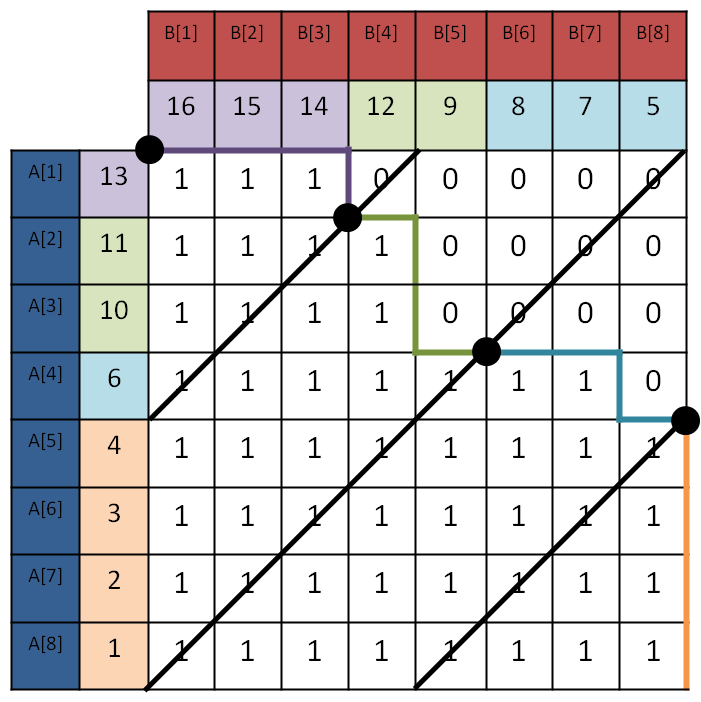
\includegraphics[width=1.0\textwidth]{images/MergePath.png}
\caption{Merge Path partitioning scheme. Figure taken from \cite{odeh2012merge}}
\label{fig:mgpu}
\end{figure}

Another interesting library that we make use of is Modern GPU, MGPU \cite{MGPU}.
More specifically we make use of its algorithm for merge sorting.
One of the primary concerns when parallel programming is how to load balance a problem across the threads.
MGPU makes use of a technique called Merge Path.
A merge sort takes in two sorted arrays, A and B, and outputs a final larger sorted array C with elements from both of the original arrays.
First, let us imagine a merge matrix, a matrix where each row corresponds to an element from A and each column represents an element from B.
If we were to try and run the merge sort sequentially, we'd start at the top left corner, and traverse the grid, moving right or down, depending on if A is greater than B at a specific element.
Merge Path realizes that a path of traversal, the so-called merge path, is formed through the merge matrix during a merge sort.
Merge Path runs diagonals through the merge matrix and find their intersection with the merge path.
All elements on the diagonal before the intersection have a less than relationship.
We can use this fact to quickly find the intersection using a binary sort.
Using the intersections of the merge path, we now know which groups of elements from A and B are responsible for specific sections of C.
If we use even divisions, we can then partition the work in a way that each thread is responsible for a constant number of elements from C.
Figure~\ref{fig:mgpu} shows an example merge matrix with a merge path and divisions.
We refer you to the original paper of \cite{odeh2012merge} for a better understanding.

There are some caveats when using these libraries.
The first is that they provide an additional dependency to your application.
Sometimes these libraries can be cumbersome to install on the host system.
The next is that it is feasible to write a higher performing code with specific knowledge of the application.
For example, knowing that part of the input array always appears in certain positions in the merged output could be utilized by the programmer.
We opt for a more general approach at the cost of some potential performance improvement.

\section{Compression}

Compression, or more specifically data compression, is a field of computer science that is rich with applications.
Compression allows us to reduce the size of the original data while still representing that original data.
Compression techniques can be categorized as either lossless or lossy.
Lossless compression tries to find repetitive or redundant patterns, while preserving all data allowing us to go back and forth from a compressed state to an uncompressed state without any data loss. 
Lossless compression is often used to archive files but is also seen in many other fields, like genetics and executables.
On the other hand, lossy compression tries to remove nonessential data from the source, often in a way that a human cannot even notice.
In turn, this allows lossy compression to compress more than any lossless compression can since it is subjective what you can or cannot notice and how much is acceptable.
Lossy compression algorithms, in contrast to lossless compression algorithms, do not preserve the original data, which now cannot be recreated.
Some of the more common lossy compression algorithms are used as codecs to reduce video or audio sizes or as graphics formats.
This includes household names like mp3 or jpeg.
The focus of our work is on the Lempel-Ziv factorization, a lossless compression algorithm.

Let's first take a step back and discuss some terminology involved in evaluating a compression algorithm.
The ratio between the sizes of the original uncompressed file and the compressed file is referred to as the \textbf{compression ratio}.
The compression ratio tells us how much smaller the file has become after compressing.
A high compression ratio indicates that the compressed file is much smaller than the original.
Next, the \textbf{compression speed} is how long it takes for a compression algorithm to run.
There is often a trade-off between the compression ratio and compression speed.
Usually, having a faster compression algorithm may result in or is caused by having a smaller compression ratio.
This works both ways.
It is important to note that different users might have different requirements, leading them to choose for one over the other.

\subsection{Lempel-Ziv}

The seminal work on the Lempel-Ziv lossless compression algorithms is the original paper authored by Lempel and Ziv in 1977 \cite{Ziv77auniversal}. 
Their work, LZ77, built their final compressed output, called the LZ77 LZ factorization, by matching with previously parsed input.
LZ77 is used in combination with Huffman coding to form the popular DEFLATE algorithm \cite{deutsch1996deflate}.
The DEFLATE algorithm is widely implemented and used; some of the most popular implementations include gzip, 7zip, zip, and the PNG file format.
Lempel and Ziv later tweaked their algorithm into LZ78 which instead provided an explicit dictionary that could be used for random lookup decompression \cite{ziv1978compression}.
LZ77 and LZ78 would become the basis for a whole family of lossless data compression algorithms.
Welch's work, LZW, improved the space efficiency of LZ78 by removing redundant characters and introducing variable encoding \cite{welch1984technique}.
LZW is used today in Unix compress and in the GIF image format.
LZSS improves on LZ77 by ensuring that the references replacing redundant symbols are indeed shorter than what they are replacing \cite{lzss}.
Today, it is used in popular archivers such as PKZip and RAR.
Other variants, including LZMA and LZSS, change some aspect of the original algorithm to increase compression speed or the compression ratio.
The focus of our thesis is on LZ77, and its LZ factorization.

Practical implementations of LZ77 use a sliding window buffer, a small section of the overall input, where the algorithm operates on a longer factored prefix and a short unfactored suffix.
In practice, using the sliding window produces comparable compression ratios while greatly increasing compression speed.
We decide to calculate the LZ factorization of the entire string instead of just a window.
In actuality, our final implementation is a compromise between these two.
Throughout the paper, we will use the terms, LZ77 LZ factorization, LZ factorization, and ideal LZ factorization.
The LZ77 LZ factorization and ideal LZ factorization refer to the LZ factorization of the whole string.
In almost all cases, the term LZ factorization will also refer to the ideal LZ factorization.
We will now describe and define the LZ factorization of a string.

\subsection{Lempel-Ziv Factorization}

\begin{table}[ht!]
\centering
\begin{tabular}{lllllllll}
i  & S{[}i{]} & nsv-lex & nsv-match & psv-lex & psv-match & LPF{[}i{]} & PrevOcc{[}i{]} & LZ \\
0  & a        & -1      & -         & -1      & 0         & -1         & 0              &    \\
1  & b        & -1      & -         & 0       & -         & 0          & -1             & 1  \\
2  & b        & 1       & b         & 0       & -         & 1          & 1              & 2  \\
3  & a        & 0       & a         & -1      & -         & 1          & 0              & 3  \\
4  & a        & 2       & -         & 0       & abb       & 3          & 0              & 4  \\
5  & b        & -1      & -         & 1       & bb        & 2          & 1              & -  \\
6  & b        & 1       & bbaa      & 2       & bb        & 4          & 1              & -  \\
7  & b        & 2       & baa       & 4       & -         & 3          & 2              & 7  \\
8  & a        & 3       & aa        & -1      & -         & 2          & 3              & -  \\
9  & a        & 3       & aab       & 8       & aa        & 3          & 3              & -  \\
10 & a        & 0       & ab        & 3       & a         & 2          & 0              & 10 \\
11 & b        & 6       & b         & 2       & ba        & 2          & 2              & -  \\
12 & a        & 10      & ab        & 3       & a         & 2          & 10             & 12 \\
13 & b        & 7       & b         & 4       & -         & 1          & 7              & - 
\end{tabular}
\caption{SA, ANSV, LPF, PrevOcc, and LZ for S = abbaabbbaaabab}
\label{tab:allsolved}
\end{table}

The LZ factorization of a string S[n] decomposes S into factors S = w1w2. . .wk where k<=n, where each factor wi is either the longest factor that appears left of wi in S or is a new character.
For example, the LZ factorization of string abbaabbbaaabab has the factorization a.b.b.a.abb.baa.ab.ab.
Various algorithms have been compared experimentally in \cite{al2012comparison}.
In general, LZ factorization algorithms all make use of a few common data structures and stages, the suffix array, the Longest Common Prefix (LCP) array, the All Nearest Smaller Values (ANSV) arrays, the Longest Previous Factor (LPF) array, and the Previous Occurrence (PrevOcc) array.
Tables~\ref{tab:allsolved} and \ref{tab:sa} shows these structures for the string abbaabbbaaabab.

\subsubsection{Suffix Array}
\label{sec:sa}

\begin{table}[ht!]
\centering
\begin{tabular}{llll}
sa & suf-lex        & nsv-lex & psv-lex \\
8  & aaabab         & 3       & -1      \\
9  & aabab          & 3       & 8       \\
3  & aabbbaaabab    & 0       & -1      \\
12 & ab             & 10      & 3       \\
10 & abab           & 0       & 3       \\
0  & abbaabbbaaabab & -1      & -1      \\
4  & abbbaaabab     & 2       & 0       \\
13 & b              & 7       & 4       \\
7  & baaabab        & 2       & 4       \\
2  & baabbbaaabab   & 1       & 0       \\
11 & bab            & 6       & 2       \\
6  & bbaaabab       & 1       & 2       \\
1  & bbaabbbaaabab  & -1      & 0       \\
5  & bbbaaabab      & -1      & 1      
\end{tabular}
\caption{Suffix array and ANSV in lexicographic order for the string abbaabbbaaabab}
\label{tab:sa}
\end{table}

The suffix array is a common data structure in string matching algorithms.
The suffix array SA of S is a lexicographic ordering array of integers of size n where each integer represents a suffix of S, so that suf\textsubscript{SA[0]} \textless suf\textsubscript{SA[1]} \textless . . . suf\textsubscript{SA[n-1]}.

First introduced as a space efficient alternative to suffix trees, the suffix array can fully replace the suffix tree with the use of additional data structures, such as the LCP array.
Suffix arrays can be used to quickly find and match strings in a dictionary.
This ability has a wide variety of applications from string searches to data compression to bioinformatics.

There exist many suffix array construction algorithms (SACA).
The skew algorithm \cite{karkkainen2003simple} uses a divide and conquer approach to construct a partial suffix array to infer the rest of the positions.
The pseudocode of the SACA that we will use is presented in figure~\ref{algorithm:sa}.
Essentially, the skew algorithm divides the suffixes into two groups.
A suffix array is constructed using the larger group, which holds 2/3 of the suffixes.
A quick check is used to see if these suffixes can be quickly sorted using their first three characters.
If this sort does not create the suffix array, due to non-unique suffixes, then the algorithm recurses until the suffix array is constructed.
The smaller group can then be sorted using inference and merged with the larger group.
Running in linear time, the skew algorithm has also been studied in parallel.
The fastest known construction of suffix arrays on the GPU by Deo and Keeley \cite{Deo} utilizes the skew algorithm.
Inspired by most of their ideas, our work is also a reimplementation and benchmark of their algorithm.

Table~\ref{tab:allsolved} shows the constructed suffix array for the string abbaabbbaaabab.
%Note that this table is in lexicographic order and not text order.

\subsubsection{LCP and LPF Array}

The LCP, longest common prefix, array is an auxiliary structure to the suffix array that provides the longest common prefix between successive suffixes in SA.
Formally, position i in the LCP array, LCP[i] = lcp(suf[SA[i-1]],suf[SA[i]]) where the lcp of two strings is the length of the common prefix between the two strings if any.
For example, the lcp(aaabab,aabab)=2.
The LCP array can be expensive to compute, but work has found that the LCP array can be constructed during the construction of the suffix array \cite{lcp}.

The LPF, longest previous factor, array holds the lengths of the longest previous factors at any position i.
In other words, LPF[i] holds the maximum lcp of suf\textsubscript{SA[i]} and all suffixes less than i.
In our example, LPF[2]=max(lcp(SA[2],SA[1]),lcp(SA[2],SA[0])).

\subsubsection{LZ Factorization Calculation}

\begin{figure}
\begin{algorithmic}[1]
\Procedure{LazyLZFactorization}{$S,n,PSV,NSV$}
\State $i \gets 1$
\While{$i \leq n$}
\State a LZ factor starts here
\If{$lcp(i,PSV) \geq lcp(i,NSV)$}
\State LZ Factor = (PSV,lcp(i,PSV))\Comment{Pair (PrevOcc,LPF)}
\Else
\State LZ Factor = (NSV,lcp(i,NSV))
\EndIf
\State if LPF = 0, PrevOcc = -1, and the character is inserted
\State $i \gets i + max(LPF,1)$\EndWhile
\EndProcedure
\end{algorithmic}
\caption{LZ Factorization Pseudocode}
\label{algorithm:lzfactorization}
\end{figure}

A naive LZ factorization algorithm may work by calculating the LPF for every position, by calculating the lcp with every previous suffix.
It can be seen that this naive algorithm runs in O(n\textsuperscript{3}) time.
This can be bounded to O(n\textsuperscript{2}) time using the knowledge that the total length of all lcp's is N.
In \cite{crochemore2008computing}, the number of positions that a suffix needs to be lcp against is reduced to the PSV and NSV.
The NSV, next smaller value, and PSV, previous smaller value, make up the ANSV, all nearest smaller values, problem.
%todo talk about why
We only need to check longer suffixes and only the closest ones since the suffix array is in lexicographic order.
Computing the ANSV problem can be done linearly and sequentially using a stack-based algorithm found in \cite{gabow1984scaling}.
By reducing the number of suffixes to compute lcp against to two, this observation now reduces the problem to an O(n) time complexity.

Table~\ref{tab:allsolved} shows the constructed suffix array and ANSV arrays (PSV,NSV) for the string abbaabbbaaabab.
We can take a look at where the NSV and PSV values for suf\textsubscript{10}=abab is found.
Simply looking at suffix array, we can see that the NSV of suf\textsubscript{10} is suf\textsubscript{0}, because 0 is the first smaller value after 10.
Likewise, the PSV of suf\textsubscript{10} is suf\textsubscript{3}, because 12, the previous value, is greater than 10, but 3, which comes before 12, is smaller.

With these NSV and PSV arrays, a naive algorithm may try and calculate the LPF for every position.
With the LPF array filled at every position, the LZ factorization can be quickly found \cite{crochemore2008computing}.
More recent LZ factorization algorithms have decided to forgo this intermediate step and directly calculate the LZ factorization.
If we examine Table~\ref{tab:allsolved}, we can see that the LZ factorization of the string abbaabbbaaabab can be reduced to 8 positions.
The positions where a factor does not begin, position 5 for example, does not need to calculate the LPF.
It also does not need to calculate the ANSV, but that calculation is relatively inexpensive and may come from the generation of the other values anyway.
Referred to as lazy LZ factorization in \cite{karkkainen2013linear}, the LPF value is only calculated at the start of a factor.
Figure~\ref{algorithm:lzfactorization} shows the basic pseudocode for calculating the LZ factorization given the PSV and NSV arrays using this lazy method.
Again, we need only check the PSV and NSV positions for the lcp and take the larger of the two.
Finally, we store the position of the larger value into the Previous Occurrence (PrevOcc) array.

The LZ factorization can be encoded simply using a sequence of pairs.
One encoding scheme uses the pair with a position of previous occurrence and the length of the match or a character (PrevOcc, LPF), if the length is 0.
The string abbaabbbaaabab encoded using this scheme would output:\\
\centerline{(PrevOcc, LPF) = [(a, 0),(b, 0),(1, 1),(0, 1),(0, 1),(2, 3),(0, 3),(10, 2)]}
Another encoding scheme uses the pair of original position and previous occurrence (LZ, PrevOcc).\\
\centerline{(LZ, PrevOcc) = [(0, a),(1, b),(2, 1),(3, 0),(4, 0),(7, 2),(10, 0),(12, 10)]}
Note that these two schemes produce the same number of pairs and each can be derived from the other.
We will now define the number of pairs in the LZ factorization to be length of the LZ factorization.
Other schemes can use different combinations of these three arrays.
For the purpose of our thesis, we need not worry about the encoding scheme, as we will output all three arrays.

\section{Related Works}

Lossless data compression on the GPU is a field that has yet to be fully investigated.
Many lossless data compression algorithms are application specific.
%“Parallel variablelength encoding on gpgpus,”

Although few, there does exist work on porting general purpose lossless data compression algorithms to CUDA.
CULZSS ports the LZSS algorithm, a sibling to LZ77, to the GPU with success \cite{ozsoy2011culzss}.
The key observation on these ports is the use of pipelining.
Most if not all of these ports split up the data to run their individual algorithm.
Many of their original algorithms allow for this.
Benefits can be found using CUDA streams, CUDA's ability to concurrently copy partial data and run kernels.
This is a feature not available in LZ factorization.
Many of these applications also make use of a sliding window, as seen in most LZ77 implementations.
%TODO
Implementations using the sliding window do not know or make use of the whole input.
This could lead to larger compressed files.

%TODO GLZSS

To the best of our knowledge, this is the first attempt to calculate the LZ factorization on the GPU.
Although we will not be calculating the ideal LZ factorization, as described later, the knowledge of the whole input string is still utilized.
The project by Shun and Zhao \cite{shun2013practical} is a multicore CPU parallel implementation of the LZ factorization.
They provide one of the first and most recent parallel implementations of the LZ factorization, where many of the inspirations throughout our project and implementation derive from.
In their project, they were able to show a O(n) work algorithm with significant speedups on a multicore CPU.
Most of our implementation matches their's, except on the GPU; however, we do not calculate the whole LPF string, and make use of the lazy LZ factorization technique described earlier.
The cost to calculate the ideal LZ factorization in a parallel fashion, as they did, was too great for GPU.
Calculating every LPF position was a very memory intensive task that we found took too long on the GPU due to the high memory latency.
This was the primary cause to the usage of the PLZ, which we'll describe in Chapter \ref{chap:implementation}.

%PLZ is like sliding window where long prefix is whole string, and suffix is chunk size

% http://delivery.acm.org.ezproxy.lib.calpoly.edu/10.1145/2380000/2379781/a5-al-hafeedh.pdf?ip=129.65.23.208&id=2379781&acc=ACTIVE%20SERVICE&key=F26C2ADAC1542D74%2E2870C5A035FC0FDB%2E4D4702B0C3E38B35%2E4D4702B0C3E38B35&CFID=343020533&CFTOKEN=37720775&__acm__=1400733002_66a60490d28a219a079b67ccd7c8315e
